\documentclass[tikz,border=10pt]{standalone}
\begin{document}
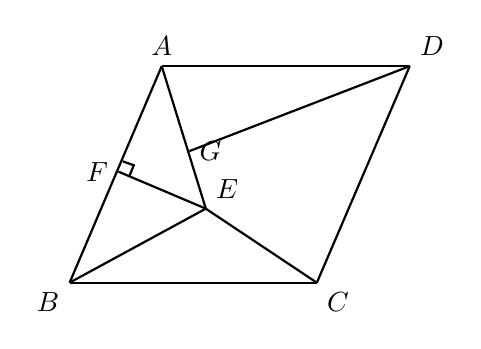
\begin{tikzpicture}[scale=1, line width=0.8pt]
  \coordinate (A) at (1.95,2.75);
  \coordinate (D) at (5.10,2.75);
  \coordinate (B) at (0.78,0);
  \coordinate (C) at (3.92,0);
  \coordinate (F) at (1.40,1.41);
  \coordinate (E) at (2.51,0.94);
  \coordinate (G) at (2.30,1.67);

  \draw (A) -- (B);
  \draw (A) -- (D);
  \draw (D) -- (C);
  \draw (B) -- (C);
  \draw (A) -- (E);
  \draw (E) -- (C);
  \draw (B) -- (E);
  \draw (F) -- (E);
  \draw (D) -- (G);

  % right angle mark at F
  \draw (1.457,1.54) -- (1.595,1.491) -- (1.538,1.351);

  \node[above] at (A) {$A$};
  \node[above right] at (D) {$D$};
  \node[below left] at (B) {$B$};
  \node[below right] at (C) {$C$};
  \node[left] at (F) {$F$};
  \node[above right] at (E) {$E$};
  \node[right] at (G) {$G$};
\end{tikzpicture}
\end{document}
